\documentclass[a4paper,10pt]{report}

% Load ``float'' before ``hyperref`` before ''algorithm``
% Note: ''algorithm`` would load ''float`` by itself
\usepackage{float}
\usepackage[pagebackref,hyperindex=true]{hyperref}

\usepackage{amsmath}
\usepackage{amssymb}
\usepackage{amsfonts}
\usepackage{amsopn}
\usepackage{braket}
\usepackage{bbm}
\usepackage{dsfont}
% \usepackage{mathabx}


% Various new commands that ease typesetting math even further
% \newcommand{\assign}{\ensuremath{\coloneq}}
% \newcommand{\rassign}{\ensuremath{\eqcolon}}
\newcommand{\assign}{\ensuremath{:=}}
\newcommand{\rassign}{\ensuremath{=:}}
\newcommand{\seteq}{\ensuremath{\overset{!}{=}}}

\newcommand{\of}[1]{\ensuremath{\left( #1 \right)}}
\newcommand{\ofs}[1]{\ensuremath{\left( #1 \right)}}

\newcommand{\norm}[1]{\ensuremath{\| #1 \|}}

\newcommand{\tmop}[1]{\ensuremath{\operatorname{#1}}}

\newcommand{\id}{\ensuremath{\mathds{1}}}
% \newcommand{\id}{\ensuremath{I}}

\newcommand{\kron}[1]{\ensuremath{\delta_{#1}}}

\newcommand{\conj}[1]{\ensuremath{\overline{#1}}}

\newcommand{\inv}{\ensuremath{{}^{-1}}}
\newcommand{\T}{\ensuremath{{}^{\textnormal{T}}}}
\newcommand{\herm}{\ensuremath{{}^{\textnormal{H}}}}

\newcommand{\tr}{\ensuremath{\textnormal{Tr}}}

\newcommand{\ft}[1]{\ensuremath{\mathcal{F}\left(#1\right)}}
\newcommand{\ift}[1]{\ensuremath{\mathcal{F}^{-1}\left(#1\right)}}

\newcommand{\fft}[1]{\ensuremath{\mathtt{FFT}\left(#1\right)}}
\newcommand{\ifft}[1]{\ensuremath{\mathtt{IFFT}\left(#1\right)}}

\newcommand{\dotp}[2]{\ensuremath{\langle #1 , #2 \rangle}}
\renewcommand{\braket}[1]{\ensuremath{\left\langle #1 \right\rangle}}

\newcommand{\bigO}[1]{\ensuremath{\mathcal{O}\left( #1 \right)}}

\newcommand{\laplace}{\ensuremath{\operatorname{\Delta}}}

\newcommand{\di}[1]{\ensuremath{\mathrm{d}#1}}
\newcommand{\diff}[3][]{\frac{\mathrm{d}^{#1}#2}{\mathrm{d}#3^{#1}}}
\newcommand{\pdiff}[2]{\frac{\partial #1}{\partial #2}}
%\newcommand{\pdiff}[3][]{\frac{\partial^{#1}#2}{\partial #3^{#1}}}
%\newcommand{\pdiffn}[3]{\frac{\partial^{#1}#2}{\partial #3^{#1}}}
% EOF

\usepackage{graphicx}
\usepackage{subfig}
\usepackage{asymptote}
\usepackage{tikz}

\usepackage[chapter]{algorithm}
\usepackage{algorithmic}

\usepackage{color}
\usepackage{relsize}
\usepackage[scaled=0.8]{beramono}
\usepackage{listings}

\definecolor{gray}{gray}{0.55}

% Python Code macro ------------------------------------------------------------

\newcommand{\python}[1] {
  \lstset{language=python,
          basicstyle=\smaller,
          basewidth=0.58em,
          columns=fixed,
          tabsize=2,
          fontadjust=true,
          frame=l,
          xleftmargin=4.2pt,
          numbers=left,
          stepnumber=2,
          breaklines=true,
          breakindent=0pt,
          prebreak=\mbox{\tiny$\searrow$},
          postbreak=\mbox{{\color{gray}$\cdots$}},
          keywordstyle=\bfseries,
          keywords={access,and,break,class,continue,def,del,elif ,else,
          except,exec,finally,for,from,global,if,import,in,is,
          lambda,not,or,pass,print,raise,return,try,while,
          True, False, None, self, from, import, as},
          numberstyle=\color{gray},
          commentstyle=\color{gray},
          stringstyle=\textit,
          showstringspaces=false,
        }
  \lstinputlisting{#1}
}

% C++ Code macro ---------------------------------------------------------------

\newcommand{\cpp}[1] {
  \lstset{language=c++,
          basicstyle=\smaller,
          basewidth=0.58em,
          columns=fixed,
          tabsize=2,
          fontadjust=true,
          frame=l,
          xleftmargin=4.2pt,
          numbers=left,
          stepnumber=2,
          breaklines=true,
          breakindent=0pt,
          prebreak=\mbox{\tiny$\searrow$},
          postbreak=\mbox{{\color{gray}$\cdots$}},
          numberstyle=\color{gray},
          commentstyle=\color{gray},
          stringstyle=\textit,
          showstringspaces=false,
        }
  \lstinputlisting{#1}
}

% Gnu R Code macro -------------------------------------------------------------

\newcommand{\gnuR}[1] {
  \lstset{language=R,
          basicstyle=\smaller,
          basewidth=0.58em,
          columns=fixed,
          tabsize=2,
          fontadjust=true,
          frame=l,
          xleftmargin=4.2pt,
          numbers=left,
          stepnumber=2,
          numberstyle=\color{gray},
          commentstyle=\color{gray},
          stringstyle=\textit,
          showstringspaces=false,
          literate={<-}{{$\leftarrow$}}1 {~}{{$\sim$}}1,
          escapeinside={(*}{*)}
        }
  \lstinputlisting{#1}
}


\usepackage[utf8x]{inputenc}
\usepackage{cancel}
\usepackage{url}
\usepackage{placeins}
\usepackage{microtype}

% Links in pdf
\usepackage{color}
\newcommand{\blue}{ \color{blue} }
\definecolor{linkcol}{rgb}{0,0,0.4}
\definecolor{citecol}{rgb}{0.5,0,0}

\hypersetup
{
colorlinks=true,
linkcolor=linkcol,
citecolor=citecol,
urlcolor=linkcol
}

% nicer backref links
\renewcommand*{\backref}[1]{}
\renewcommand*{\backrefalt}[4]{%
\ifcase #1 %
(Not cited.)%
\or
(Cited on page~#2.)%
\else
(Cited on pages~#2.)%
\fi}
\renewcommand*{\backrefsep}{, }
\renewcommand*{\backreftwosep}{ and~}
\renewcommand*{\backreflastsep}{ and~}

\parindent 0cm

\newcommand{\clearemptydoublepage}{\newpage{\pagestyle{empty}\cleardoublepage}}


\begin{document}

\begin{titlepage}
\begin{center}
  \hfill
  \vspace{2.0cm}

  { \huge\textsc{\LARGE A fast C++ Template library for Total Variation Minimization of manifold-valued 
  two- and three-dimensional images\\[10pt]
  }}
  	~\\[20pt]
	
   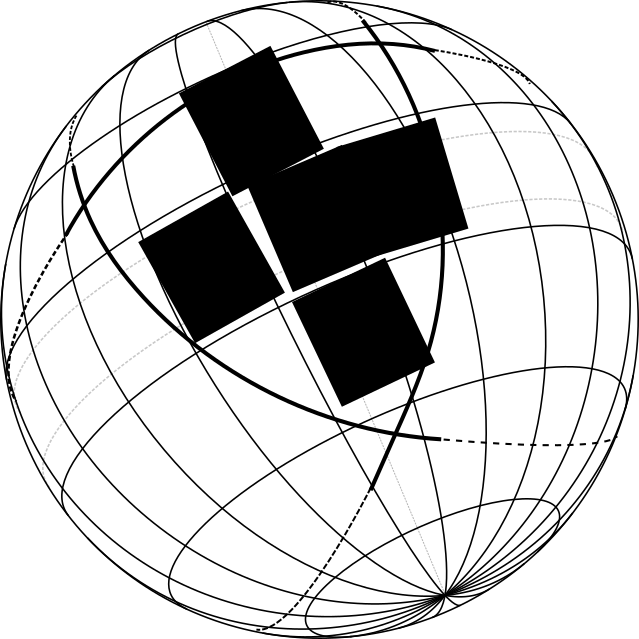
\includegraphics[width=0.5\linewidth]{./figures/title/mtvmtl.pdf}
	
	~\\[20pt]

  {\huge{Master Thesis}}\\[2.5cm]

  {\emph{written by}}\\
  {\large Pascal Debus}
  \\[0.6cm]
  {\emph{supervised by}}\\
  Markus Sprecher{\emph{,}}\\
  Prof. Dr. Philipp Grohs\\

  Seminar for Applied Mathematics\\
  ETH Zurich
  \\[0.5cm]
  {October 1, 2015}
\end{center}
\begin{tikzpicture}[remember picture,overlay]
   \node[anchor=north west,inner sep=40pt] at (current page.north west)
              {\includegraphics[scale=0.15]{./figures/title/ETHlogo.png}};
   \node[anchor=south east,inner sep=40pt] at (current page.south east)
              {\includegraphics[scale=0.25]{./figures/title/sam_logo.png}};
\end{tikzpicture}
\end{titlepage}



\clearemptydoublepage

\tableofcontents
\listoffigures
%\listofalgorithms

\clearemptydoublepage

\begin{chapter}{Introduction}
\label{ch:introduction}
Various forms of noise occur in many forms of data acquisiation, transmission and processing.y
This noise needs to be removed in order to obtain a meaningful interpretation of the data, to enable further processing or, as in many image processing 
applications, just for aesthetical reasons. A common everyday example for a noisy image is taking a picture with a digital camera (e.g. integrated in a smart phone) in a weakly illuminated room:
Especially the dark areas of the picture are not uniform in color and brightness but have small variations from pixel to pixel.\\

A noise removal algorithm needs to remove these small variations but at the same time not alter important features of the data. In the case of images important features are for example 
the edges separating areas of different colors and providing the necessary sharpness of the picture. These edges on the other hand are characterized by large variations. This distinction
between small and large variations is also helpful in the task of inpainting, which tries to restore the picture at unknown or damaged regions.\\

The method of total variation(TV) noise removal, which has the above described capabilities, was first introduced by Rudin, Osher and Fatemi \cite{RudinOsher} in 1992
for the case of real-valued, that means grayscale images. Their method is briefly summarized in the following section.

\section{Grayscale images}
Let $u_0: \Omega\subset \mathbb{R}\to \mathbb{R}$ desribe the original, noise-free image, where the image domain $\Omega$ is usually a rectangular or cuboid subset of $\mathbb{R}^2$ or $\mathbb{R}^3$, respectively. 
Assuming the original pictures is corrupted by gaussian noise $n: \Omega\to\mathbb{R}$ with zero mean and variance $\sigma^2$ the noisy picture is given by $u: \Omega\to \mathbb{R}$, where
$u = u_0 + n$. The edge preserving denoising of the picture is then equivalent to the solution $u^* :\Omega\to \mathbb{R}$ of the following constrained optimization problem:
\begin{align}
    \label{osher_opt}
    u^* &= \operatorname{argmin}_{f: \Omega\to \mathbb{R}}\int_\Omega\left\vert\nabla u\right\vert  \quad\text{s.t.}\\
    \int_\Omega(u-u_0) &= 0, \quad\text{and} \int_\Omega(u-u_0)^2 = \sigma^2
\end{align}

The first term $TV(u)=\int_\Omega\left\vert\nabla u\right\vert$ is called the total variation of $u$. Rudin, Osher and Fatemi then use a partial differential equation (PDE) approach to solve
the corresponsing Euler-Lagrange equation for (\ref{osher_opt}). Later Chambolle and Lions \cite{ChambolleLions} showed that (\ref{osher_opt}) is equivalent to the minimization of
the functional
\begin{equation}
    \label{osher_func}
    \frac{1}{2}\norm{u-u_0}_2^2 +\lambda \int_\Omega\left\vert\nabla u\right\vert
\end{equation}

\subsection{Edge preservation} % (fold)
\label{sub:Edge preservation}
A basic intuition why the $L^1$ norm in (\ref{osher_func}) is besser suited for conserving sharp discontinuities such as edges can be seen from the following plot.\\

\begin{figure}[h!]
        \centering
	    \includegraphics[width=0.9\linewidth]{./figures/introduction/tv12comparison.pdf}
	\caption[Comparison total variation]{Plots of three functions with ($N=1,\;10,\;100$) steps and a total variation equal to $1.0$}
	\label{fig:tv12comparison}
\end{figure}
\begin{table}[h!]
\centering
\begin{tabular}{|l|l|l|}
    \hline
    \textbf{Function} & $\int_{[0,1]}\left\vert\nabla f\right\vert$ & $\int_{[0,1]}\left\vert\nabla f\right\vert^2$ \\
    \hline
    $f_1$ & 1.0 & 1.0 \\
    $f_2$ & 1.0 & 0.1 \\
    $f_3$ & 1.0 & 0.01 \\
    \hline
\end{tabular}
\end{table}

One can see that the $L^2$ variation term favors continuous transitions such as $f_3$ rather than the sudden jump in $f_1$ whereas the total variation is the same for
all cases.
% subsection Edge preservation (end)

\section{Color Images}
The next step in the development of image denoising algorithms was their generalization to color images. From a mathemtical perspective this just means considering pictures
from $\Omega\to C\simeq \mathbb{R}^3$ where the form and additional properties of $C$ depend on the chosen color model. \\
In the most simple case of linear models, like RGB for instance, one could choose $C$ as $[0,1]^3$ and consider denoising each component individually (channel-by-channel model)
or consider $\mathbb{R}^3$ as a normed vector space of tuples $(x_R, x_G, x_B)$ (linear-vectorial model).\\
For the nonlinear models, especially the so-called chromaticity-brightness model, Chang and Kang \cite{ChangKuang} showed the closest resemblance to human perception.
In this case we can take $C=S^2\times [0,1]$ such that the chromatictiy takes values on the sphere $S^2$ considered as a submanifold of the euclidian space $\mathbb{R}^3$, 
while the brightness is real-valued, as in the case of graysale images.

\section{Manifold-valued Images} % (fold)
\label{sec:Manifold-valued Images}
In the last section we have already seen that, depending on the chosen color model, pixels can take their values on a manifold and are usually represented by their matrices.
This data arises in a variety of application such as Diffusion Tensor Magnetic Resonance Imaging (DTI-MRI), computer vision and robotics to name just a few.

\section{Objective and Outline of this work}
In this work we will introduce an extendable multi-threaded C++ template library for the purpose of TV Minimization of manifold-valued images. 
So far the implemented minimization algorithms are based on the iteratively reweighted least squares (IRLS) adaption suggested by Sprecher and Grohs \cite{SprecherIRLS} as well as a 
proximal point algorithm by Weinmann et al \cite{WeinmannPRPT}. We extend the implementation to 3D images cubes, the Grassmann manifold and also provides some quasi-analytic expressions
for derivatives of the Riemannian distance function.\\

In the following chapter 2 a short summary of the necessary theory, a description of the algorithms and relevant properties for each of the implemented manifolds.
After that the chapter 3 introduces the library itself in particular its capabilieties, design concepts, structure, installation and usage in the form of some typical
use cases. In Chapter 4 numerical experiments are conducted, showing various application of the library as well as convergence behavior and comparisons between 
IRLS and proximal point based minimizers.\\

Finally, chapter 5 concludes with possible extensions and adaptions of the library, in particular possibility of recursive splitting of the image domain into smaller subproblems and
the transition to distributed architectures.
% section Manifold-valued Images (end)
\end{chapter}


\clearemptydoublepage

\begin{chapter}{Theory}
\label{ch:theory}

\section{Riemannian Newton Method} % (fold)
\label{sec:Riemannian Newton Method}

% section Riemannian Newton Method (end)

\section{Algorithms} % (fold)
\label{sec:Algorithms}

\subsection{IRLS} % (fold)
\label{sub:IRLS}

% subsection IRLS (end)

\subsection{Proximal Point} % (fold)
\label{sub:Proximal Point}

% subsection Proximal Point (end)

% section Algorithms (end)

\section{Manifolds} % (fold)
\label{sec:Manifolds}

\subsection{Euclidian} % (fold)
\label{sub:Euclidian}

% subsection Euclidian (end)

\subsection{Sphere $S^n$} % (fold)
\label{sub:Sphere}

% subsection Sphere (end)

\subsection{Special Orthogonal Group SO(n)} % (fold)
\label{sub:SO(N)}

\subsubsection{Second derivatives of the distance function} % (fold)
\label{ssub:Second derivatives of the distance function}
For the computation of the second derivatives we can take the expression obtained using the above theorem as a starting point and follow the approach and notation of Magnus \cite{magnus}. 
This allows us to express the derivatives as combinations of simple Kronecker product of the arguments which also is very straightforward and compact to implement. 
The detailed derivations can be found in the appendix \ref{appendix} while here we only represent the final results. \\
For the second derivative with respect to the first argument one readily arrives at
\begin{equation}
    \label{eq:son_xx_der}
    \frac{\partial^2 d^2(X,Y)}{\partial X\partial X} = -2\left[\left(\left(\log X^TY\right)^T\otimes\mathbbm{1}_n\right) + \left(\mathbbm{1}_n\otimes X \right)\operatorname{D}\log(X^TY) \left(Y^T\otimes\mathbbm{1}_n \right) K_{nn}\right],
\end{equation}
where $K_{nn}$ denotes the commutator matrix which transforms the columnwise vectorization of a matrix $A$ to the vectorization of its tranpose $A^T$.\\

The mixed derivative is given by
\begin{equation}
    \label{eq:son_xy_der}
    \frac{\partial^2 d^2(X,Y)}{\partial X\partial Y} = -2\left(\mathbbm{1}_n\otimes X \right)\operatorname{D}\log(X^TY) \left(\mathbbm{1}_n\otimes X^T \right),
\end{equation}
These expressions are quasi-analytical: Matrix logarithms, exponentials and the Frechet derivative of the logarithms need to be evaluated numerically. Details concerning the 
implementation of the latter are postponed to section \ref{seq:frechetderivatives}.

% subsubsection Second derivatives of the distance function (end)


% subsection SO(N) (end)

\subsection{Symmetric Positive Definite Matrices SPD(n)} % (fold)
\label{sub:SPD(N)}

\subsubsection{Second derivatives of the distance function} % (fold)
\label{ssub:Second derivatives of the distance function}
For the SPD matrices we proceed in the same way as for the orthogonal group and obtain
\begin{align}
    \label{eq:spd_xx_der}
    \frac{\partial^2 d^2(X,Y)}{\partial X\partial X} &= 
    2\Bigg[
	\left(X^{-\frac{1}{2}}\log\left(X^{-\frac{1}{2}}YX^{-\frac{1}{2}}\right)^T\otimes\mathbbm{1}_n\right)
	+\left(\mathbbm{1}_n\otimes X^{-\frac{1}{2}}\log\left(X^{-\frac{1}{2}}YX^{-\frac{1}{2}}\right)\right) \\
    &	+\left(X^{-\frac{1}{2}}\otimes X^{-\frac{1}{2}}\right)\operatorname{D}\log(X^{-\frac{1}{2}}YX^{-\frac{1}{2}})\left( \left(X^{-\frac{1}{2}}Y\otimes\mathbbm{1}_n\right)
	+ \left(\mathbbm{1}_n\otimes X^{-\frac{1}{2}}Y\right)\right) 
    \Bigg] \times\cdots \nonumber \\
    & \cdots\times\left(X^{-\frac{1}{2}}\otimes X^{-\frac{1}{2}}\right)\operatorname{D}(X^{\frac{1}{2}})\nonumber
\end{align}
and for the mixed derivatives
\begin{equation}
    \label{eq:spd_xy_der}
    \frac{\partial^2 d^2(X,Y)}{\partial X\partial Y} = -2\left(X^{-\frac{1}{2}}\otimes X^{-\frac{1}{2}}\right)\operatorname{D}\log\left(X^{-\frac{1}{2}}Y X^{-\frac{1}{2}}\right)\left(X^{-\frac{1}{2}}\otimes X^{-\frac{1}{2}}\right)
\end{equation}

% subsubsection Second derivatives of the distance function (end)

% subsection SPD(N) (end)

\subsection{Grassmanian Gr(n,p)} % (fold)
\label{sub:Grassmanian}
The Grassmann manifold is special among the manifolds so far considered due to the fact that it is a quotient manifold. 
As such, there are different possbilieties for choosing equivalence classes and representatives thereof from some matrix space that need to be addressed
before an implementation.\\

For positive integers $n$ and $p\leq n$ the Grassmann manifold is defined as the set of $p$-dimensional linear subspaces of $\mathbb{R}^n$. 
Since a linear subspace $\mathcal{Y}\in Gr(n,p)$ can be specified using a basis, we can arrange its basis vectors as columns of
a matrix $Y\in\mathbb{R^{n\times p}}$ such that its column space spans $\mathcal{Y}$. The rank of $Y$ must necessarily be full and equal to $p$ because of the linear independence
of its columns. Hence, elements of $Gr(n,p)$ can be represented using elements of the \emph{non-compact Stiefel manifold}
\begin{equation}
    \tilde St(n,p) := \left\lbrace Y\in\mathbb{R}^{n\times p}:\; \operatorname{rank}Y=p\right\rbrace.
\end{equation}

\subsubsection{Quotient representations} % (fold)
\label{ssub:Quotient representations}
Observing now that post-multiplication by any invertible $G\in Gl(p)$ does not change the span of $Y$, we can form the equivalence classes
\begin{equation}
    Y\,GL(p) := \left\lbrace YG: G\in Gl(p)\right\rbrace
\end{equation}
consisting of all matrices having the same span as $Y$. These equivalence classes can be thought of as the distinct elements of the Grassmannian which
leads to the following quotient manifold representation.\\
\begin{equation}
    Gr(n,p):=\tilde St(n,p) / Gl(p)
\end{equation}

This representation used by Absil et al\cite{AbsilGrasmman} which is very general because only the rank is specified. In the next steps of presenting the relavant quantities for the
algorithm we will follow Absil's derivation and notation but choose the quotient representation used by Edelman et al \cite{EAS} which is based on the orthogonal group. This will simplify the
most expressions and is also desirable from an algorithmic point of view as it removes more degrees of freedom in the choice of possbily unique representatives.\\

For the sake of completeness we also mention a completely different approach by Sato and Iwai \cite{SatoIwai} who choose $\mathbb{R}^{n\times n}$ as embedding space
where elements of $Gr(n,p)$ are given by rank $p$ orthogonal projection matrices. The presented application are, however, mostly eigenvalue problems while in the case
of image denoising the increased memory requirements are disadvantageous.\\

The orthogonal group quotient represenation of the Grassmann manifold is given by
\begin{equation}
    Gr(n,p) = St(n,p) / O(p) %= O(n) / (O(p) \times O(n-p)),
\end{equation}
where we denote by $St(n,p)=\left\lbrace Y\in\mathbb{R}^{n\times p}:\; Y^TY=\mathbbm{1}_p,\right\rbrace$ the \emph{compact} Stiefel manifold with the additional
requirement that the basis spanning the subspace $\mathcal{Y}$ be orthonormal now. The canoncial quotient projection map is then given by
\begin{equation}
    \pi : St(n,p)\ni Y \mapsto \operatorname{span} Y=\mathcal{Y} \in Gr(n, p)
\end{equation}
% subsubsection Quotient representations (end)

\subsubsection{Locally unique representatives} % (fold)
\label{ssub:Locally unique Representative}
Let $U\in St(n,p)$ and define the local affine cross section through $U$ and orthogonal to the fiber $U[O(p)]=\pi^{-1}(\mathcal{U})\subset St(n,p)$ by
\begin{equation}
    S_U := \left\lbrace V\in St(n,p): U^T(V-U)=0 \right\rbrace\subset St(n,p).
\end{equation}

The equivalence class of $V\in St(n,p)$ is equal to $\pi^{-1}(\pi(V))=V\,O(p)$ and to calculate its intersection with $S_U$ we choose $R\in O(p)$ such that
$VR\in VO(p)$ and obtain
\begin{align}
    VR\in S_U\;\Leftrightarrow\; U^T(VR-U)=0 \;\Leftrightarrow\; R = (U^TV)^{-1}
\end{align}
which leads to the intersection
\begin{align}
    S_U \cap V[O(p)] = \left\lbrace VR = V(U^{T}V)^{-1} \right\rbrace .
\end{align}
which can be also empty if $U^{T}S$ is not invertible. Finally, we define a \emph{cross-section mapping} $\sigma_U$ restricted to the set
\begin{equation}
    \mathcal{U}_U := \left\lbrace\mathcal{V}=\operatorname{span}V:\; U^TV\in GL(p) \right\rbrace
\end{equation}
by 
\begin{equation}
    \sigma_U: Gr(n,p)\supset \mathcal{U}_U\ni\mathcal{V}=\operatorname{span}V\mapsto V(U^{T}V)^{-1} \in S_U \subset St(n,p).
\end{equation}
which is a diffeomorphism providing the differentiable structure considering the embedding of $St(n,p)$ in Euclidian space.\\

The above considerations are important for the design of algorithms for two reasons.\\
Firstly, it provides the means to give well-defined expressions for various quantities we want to compute using arbitrary representatives.
For the case of an average for instance, we can take representatives $Y_1,\ldots,Y_n\in St(n,p)$ for $\mathcal{Y}_1,\ldots,\mathcal{Y}_n\in Gr(n,p)$
and find a $U\in St(n,p)$ such that $S_U$ has non-zero intersection with all the $Y_i$'s equivalence classes, which is equivalent
to $U^TY_i\in Gl(p)$. The average $\mathcal{A}$ can then be written as
\begin{equation}
    \mathcal{A} := \pi\left(\sum_{i=1}^{n}\sigma_U(Y_i)\right)=\pi\left(\sum_{i=1}^{n}Y_i(U^{T}Y_i)^{-1}\right).
\end{equation}

Secondly, it allows us to find a parametrization of $Gr(n,p)$ in terms of $\mathbb{R}^{n\times p}$ matrices. This is necessary to construct a local basis of the tangent base
and make the dimension of the sparse linear system a function of the intrinsic manifold dimension $(n-p)p$ instead of the embedding dimension $np$.
% subsubsection Locally unique Representative (end)

\subsubsection{Tangent space} % (fold)
\label{ssub:Tangent space}
Due to the quotient structure which forces us to work with representatives we cannot just use the usual method for finding the tangent space by differentiating
curves on the manifold but have to start with "numerator" of the quotient $St(n,p)$ instead. For the Grassmann manifolds only tangent vectors of a special subspace of $T_YSt(n,p)$,
the horizontal space, can modify the span of subspace and exactly those belong to the tangent space of $Gr(n,p)$. \\

Let $Y\in St(n,p)\subset\mathbb{R}^{n\times p}$. Then tangent space at $Y$ (\cite{AbsilOptim} for details of the derivation) to the compact Stiefel manifold is given by
\begin{align}
    \label{eq:stiefel_tangentspace}
   T_YSt(n,p)	&= \left\lbrace Z\in\mathbb{R}^{n\times p}: Y^TZ+Z^TY=0 \right\rbrace\\
   &=  \left\lbrace Y\Omega + Y_{\bot}K: \Omega\in\operatorname{Skew}(p),\, K\in\mathbb{R}^{(n-p)\times p} \right\rbrace\nonumber
\end{align}
where $Y_{\bot}\in\mathbb{R}^{(n\times (n-p)}$ is defined such that $[Y,Y_{\bot}]\in O(n)$. The second representation of (\ref{stiefel_tangentspace})
already implies the decomposition into vertical and horizontal spaces we are going to perform next.

The vertical space at $Y$ is by definition the tangent space to the fiber $\pi^{-1}(\pi(Y))$
\begin{equation}
    \label{eq:stiefel_horizontalspace}
    V_Y = T_Y\pi^{-1}(\pi(Y))=T_YY[O(p)]=Y[\operatorname{Skew}(p)],
\end{equation}
while the horizontal space is defined as its orthogonal complement with respect to (\ref{eq:stiefel_tangentspace})
\begin{equation}
    \label{eq:stiefel_verticalspace}
    H_Y=V_Y^{\bot} =\left\lbrace H\in T_Y St(n,p):Y^TH=0 \right\rbrace \simeq Y_{\bot}[\mathbb{R}^{(n-p)\times p}].
\end{equation}

Using this, the tangent space to $Gr(n,p)$ at $\pi(Y)=\mathcal{Y}$, along with its projector is given by 
\begin{align}
    \label{eq:grassmann_tangentspace}
    T_{\mathcal{Y}}Gr(n,p)&\simeq  H_YSt(n,p)\simeq Y_{\bot}[\mathbb{R}^{(n-p)\times p}]\\
    \pi_{Y_{\bot}}&:=\mathbbm{1}_n-YY^T
\end{align}


% subsubsection Tangent space (end)

\subsubsection{Exponential map} % (fold)
\label{ssub:Exponential map}
Let $X, Y$ span $\mathcal{X}, \mathcal{Y}$, respectively and let $U\Sigma V^{T}$ denote the compact singular value decomposition of $Y$. Then
\begin{equation}
    \operatorname{Exp}_{\mathcal{X}}(\mathcal{Y})=\operatorname{span}\left( XV\cos\Sigma + U\sin\Sigma\right).
\end{equation}
% subsubsection Exponential map (end)



\subsubsection{Distance function} % (fold)
\label{ssub:Distance function}
Using the previously defined exponential map, one can easily define a geodesic distance function on the Grassmann manifold which is induced by its Riemannian metric
\begin{equation}
    g(X,Y) = \tr X^TY
\end{equation}
Then the distance function is given by the principal angles $\theta_i$ between the subspaces 
\begin{equation}
    \label{eq:gr_geod_dist}
    d_g^2(X,Y) = \norm{\theta}_2^2=\sum_{i=1}^p\theta_i^2,
\end{equation}
where the the principal angles can be obtained by computing the singular value decomposition of $X^TY$.

\begin{align}
    X^TY &= U\Sigma V^T = U\cos\Theta V^T\\
    \Sigma &= \operatorname{diag} (\sigma_1,\cdots,\sigma_p)\\
    \Theta &= \operatorname{diag} (\theta_1,\cdots,\theta_p) = \operatorname{diag} (\arccos\sigma_1,\cdots,\arccos\sigma_p)
\end{align}

The distance function (\ref{eq:gr_geod_dist}) has the disadvantage that due to the occurence of the cosine no analytic derivatives can be computed.\\

To avoid this problem, we follow Absil's \cite{absil_GR} approach and choose an equivalent norm, the so-called projection Frobenius norm, given by

\begin{equation}
    d_P^2(X,Y) = \frac{1}{2}\norm{XX^T-YY^T}_{F}^{2} = \sum_{i=1}^p\sin^2\theta_i
\end{equation}


% subsubsection Distance function (end)


\subsubsection{First derivatives of the distance function} % (fold)
\label{ssub:First derivatives of the distance function}

\begin{equation}
    \label{eq:gr_x_der}
    \frac{\partial d^2(X,Y)}{\partial X} = 2\left(XX^T-YY^T\right)X
\end{equation}


% subsubsection First derivatives of the distance function (end)

\subsubsection{Second derivatives of the distance function} % (fold)
\label{ssub:Second derivatives of the distance function}

\begin{equation}
    \label{eq:gr_xx_der}
    \frac{\partial^2 d^2(X,Y)}{\partial X\partial X} = 2
    \left[
	\left(X^TX\otimes \mathbbm{1}_{n}\right) 
	+ \left(\mathbbm{1}_p\otimes (XX^T-YY^T)\right)
	+ \left(X^T\otimes X\right)K_{np}
    \right]
\end{equation}

The mixed derivative is given by
\begin{equation}
    \label{eq:gr_xy_der}
    \frac{\partial^2 d^2(X,Y)}{\partial X\partial Y} = -2\left[\left(X^TY\otimes \mathbbm{1}_{n}\right) + \left(X^T\otimes Y\right)K_{np}\right]
\end{equation}


% subsubsection Second derivatives of the distance function (end)


% subsection Grassmanian Gr(N,P) (end)

% section Manifolds (end)

\section{Fr\'{e}chet derivatives of matrix logarithm and square root} % (fold)
\label{sec:frechetderivatives}
To use the derivative expression computed above we need the so called Kronecker form of the Fr\'{e}chet derivative. The Fr\'{e}chet derivative
of a matrix valued function $f:\mathbb{R}^{n\times n}\to\mathbb{R}^{n\times n}$ at a point $X\in\mathbb{R}^{n\times n}$ is a linear function mapping $E\in\mathbb{R}^{n\times n}$
to $L_f(X,E)\in \mathbb{R}^{n\times n}$ such that
\begin{equation}
    f(X+E) - f(X) - L_f(X,E) = \mathcal{o}(\norm{E}).
\end{equation}
Chain rule and inverse function theorem also hold for the Fr\'{e}chet derivative:
\begin{align}
    L_{f\circ g}(X, E) &= L_{f}(g(X)),L_{g}(X,E))\\
    L_{f}(X, L_{f^{-1}}(f(X),E)) &= E
\end{align}

As we did in our formulation of the derivatives of the distance function, it can also be represented in the Kronecker form in which is represented as map
$K_f:\mathbb{R}^{n^2}\to\mathbb{R}^{n^2}$, such that $K_f(X)\in \mathbb{R}^{n^2\times n^2}$ is defined by
\begin{equation}
    \label{eq:kronckerform}
    \operatorname{vec}(L_f(X,E))=K_f(X)\operatorname{vec}(E)
\end{equation}
where $\operatorname{vec}:\mathbb{R}^{n\times n}\to\mathbb{R}^{n^2}$ denotes the columnwise vectorization operator.

\subsection{Derivative of the matrix square root} % (fold)
\label{sub:Derivative of the matrix square root}
We start by considering the Fr\'{e}chet derivative of $f(X)=X^2$, which is given by
\begin{equation}
    L_{X^2}(X,E) = XE + EX.
\end{equation}
Applying the inverse function theorem consequently leads to
\begin{equation}
    L_{X^2}(X^{\frac{1}{2}},L_{X^{\frac{1}{2}}}(X,E))=X^{\frac{1}{2}}L_{X^{\frac{1}{2}}}(X,E) + L_{X^{\frac{1}{2}}}(X,E)X^{\frac{1}{2}} = E,
\end{equation}
where the last equality shows that the Fr\'{e}chet derivative of the matrix square root $L_{X^{\frac{1}{2}}}(X,E)$ satisfies the Sylvester equation 
\begin{equation}
    \label{eq:sylvester}
    X^{\frac{1}{2}}L + LX^{\frac{1}{2}} = E,\quad L:=L_{X^{\frac{1}{2}}}(X,E).
\end{equation}

The Kronecker representation $K_{X^{\frac{1}{2}}}$ can now be obtained be using the vectorization operator on both sides of the equation and rearrange the term
to the form (\ref{eq:kronckerform}) which leads to
\begin{equation}
    K_{X^{\frac{1}{2}}}(X)=\left[\left(\mathbbm{1}\otimes X^{\frac{1}{2}}\right)+\left(X^{\frac{1}{2}T}\otimes \mathbbm{1}\right) \right]^{-1}.
\end{equation}
However, this straightforward approach has the disadvantage that the inverse of a $n^2\times n^2$ matrix need to be computed which has complexity
$\mathcal{O}((n^2)^3)=\mathcal{O}(n^6)$. In addition to that, the inverse needs to be found explicitly which is not numerically stable in general.\\

The Sylvester equation (\ref{eq:sylvester}), on the other hand, can be solved with $\mathcal{O}(n^3)$ operations via Schur transformation. We choose $E^{ij}$, the single-entry
matrices having 1 at $(i,j)$ and zero everywhere else, as a basis for $\mathbb{R}^{n\times n}$ and solve the Sylvester equation for each of the $n^2$ 
basis matrix elements. By that, the total complexity can be reduced to $n^2\mathcal{O}(n^3)=\mathcal{O}(n^5)$ and we avoid the 
potentially problematic explicit computation of inverses altogether.\\

We then obtain the final Kronecker form of the derivative by constructing its rows from the vectorized, tranposed Fr\'{e}chet derivatives:
\begin{equation}
    \left(K_{X^{\frac{1}{2}}}\right)_{in + j,\cdot} = \operatorname{vec}\left(L_{X^{\frac{1}{2}}}(X,E^{ij})^T\right) 
\end{equation}

\subsection{Derivative of the matrix logarithm} % (fold)
\label{sub:Derivative of the matrix logarithm}
For the logarithm we follow the approach described by Al-Mohy et al \cite{almohy_frechetlog} which is based on the differentiation of the Pad\'{e} approximant to $\log(1+X)$.
Since this is only applicable if the norm of $X$ is sufficiently small, the  use of an inverse scaling and squaring technique based on the relation
\begin{equation}
    \log(X) = 2\log(X^{\frac{1}{2}})
\end{equation}
is necessary.\\

Application of the chain rule leads to
\begin{equation}
    L_{\log}(X,E_0) = 2\log\left(X^{\frac{1}{2}},L_{X^{\frac{1}{2}}}(X,E_0)\right).
\end{equation}
The second argument on the right hand side can again be written as solution $E_1:=L_{X^{\frac{1}{2}}}(A,E_0)$ of an Sylvester-type equation
\begin{equation}
    X^{\frac{1}{2}}E_1+E_{1}X^{\frac{1}{2}}=E_0.
\end{equation}
Repeating the procedure $s$ times results in
\begin{align}
    L_{\log}(X,E_0)&=2^sL_{\log}\left(X^{\frac{1}{2^s}},E_s\right)\\
    X^{\frac{1}{2^{i}}}E_i+E_iX^{\frac{1}{2^{i}}}&=E_{i-1},\quad i=1,\ldots,s
\end{align}
where $E_s$ is obtained by successivly solving the set of Sylvester equations defined in the second line.\\

Finally, the Pad\'{e} approximant of order $m$ in its partial fraction form \cite{highham_pade} is given by
\begin{equation}
    \label{eq:pade_log}
    r_m(X) = \sum_{j=1}^{m}\alpha_j^{(m)}(\mathbbm{1}+\beta_j^{(m)}X)^{-1}X
\end{equation}
where $\alpha_{j}^{(m)},\beta_{j}^{(m)}\in (0,1)$ are the $m$-point Gauss-Legendre quadrature weights and nodes.\\

The derivative of (\ref{eq:pade_log}) is then easily computed as 
\begin{equation}
    L_{r_m}(X,E) = \sum_{j=1}^m\alpha_j^{(m)}(\mathbbm{1}+\beta_j^{(m)}X)^{-1}E(\mathbbm{1}+\beta_j^{(m)}X)^{-1}
\end{equation}
which leads to the final approximation of the matrix logarithm derivative, 
\begin{equation}
    \label{eq:dlog_approx}
    L_{\log}(X,E)\approx 2^{s}L_{r_m}\left(X^{\frac{1}{2^s}}-\mathbbm{1},E_s \right).
\end{equation}

For the implementation of (\ref{eq:dlog_approx}) we use algorithm 5.1 from \cite{almohy_frechetlog} with fixed $m=7$.
The Kronecker representation is then constructed as in the square root case.
% subsection Derivative of the matrix logarithm (end)




% subsection Derivative of the matrix square root (end)


% section Frechet derivative of the matrix logarithm and square root (end)


\end{chapter}


\clearemptydoublepage

%\input{./ch_analytic_solution.tex}

%\clearemptydoublepage

%\input{./ch_ladder_operators.tex}

%\clearemptydoublepage

%\input{./ch_parameters.tex}

%\clearemptydoublepage

\appendix
%\input{./ap_integrals.tex}

%\clearemptydoublepage

\bibliographystyle{plain}
\bibliography{mt}

\end{document}
